\providecommand{\main}{../../../..}
\documentclass[\main/dresen_thesis.tex]{subfiles}
\begin{document}
  \label{sec:doubleLayers:vsm}

  \begin{figure}[tb]
    \centering
    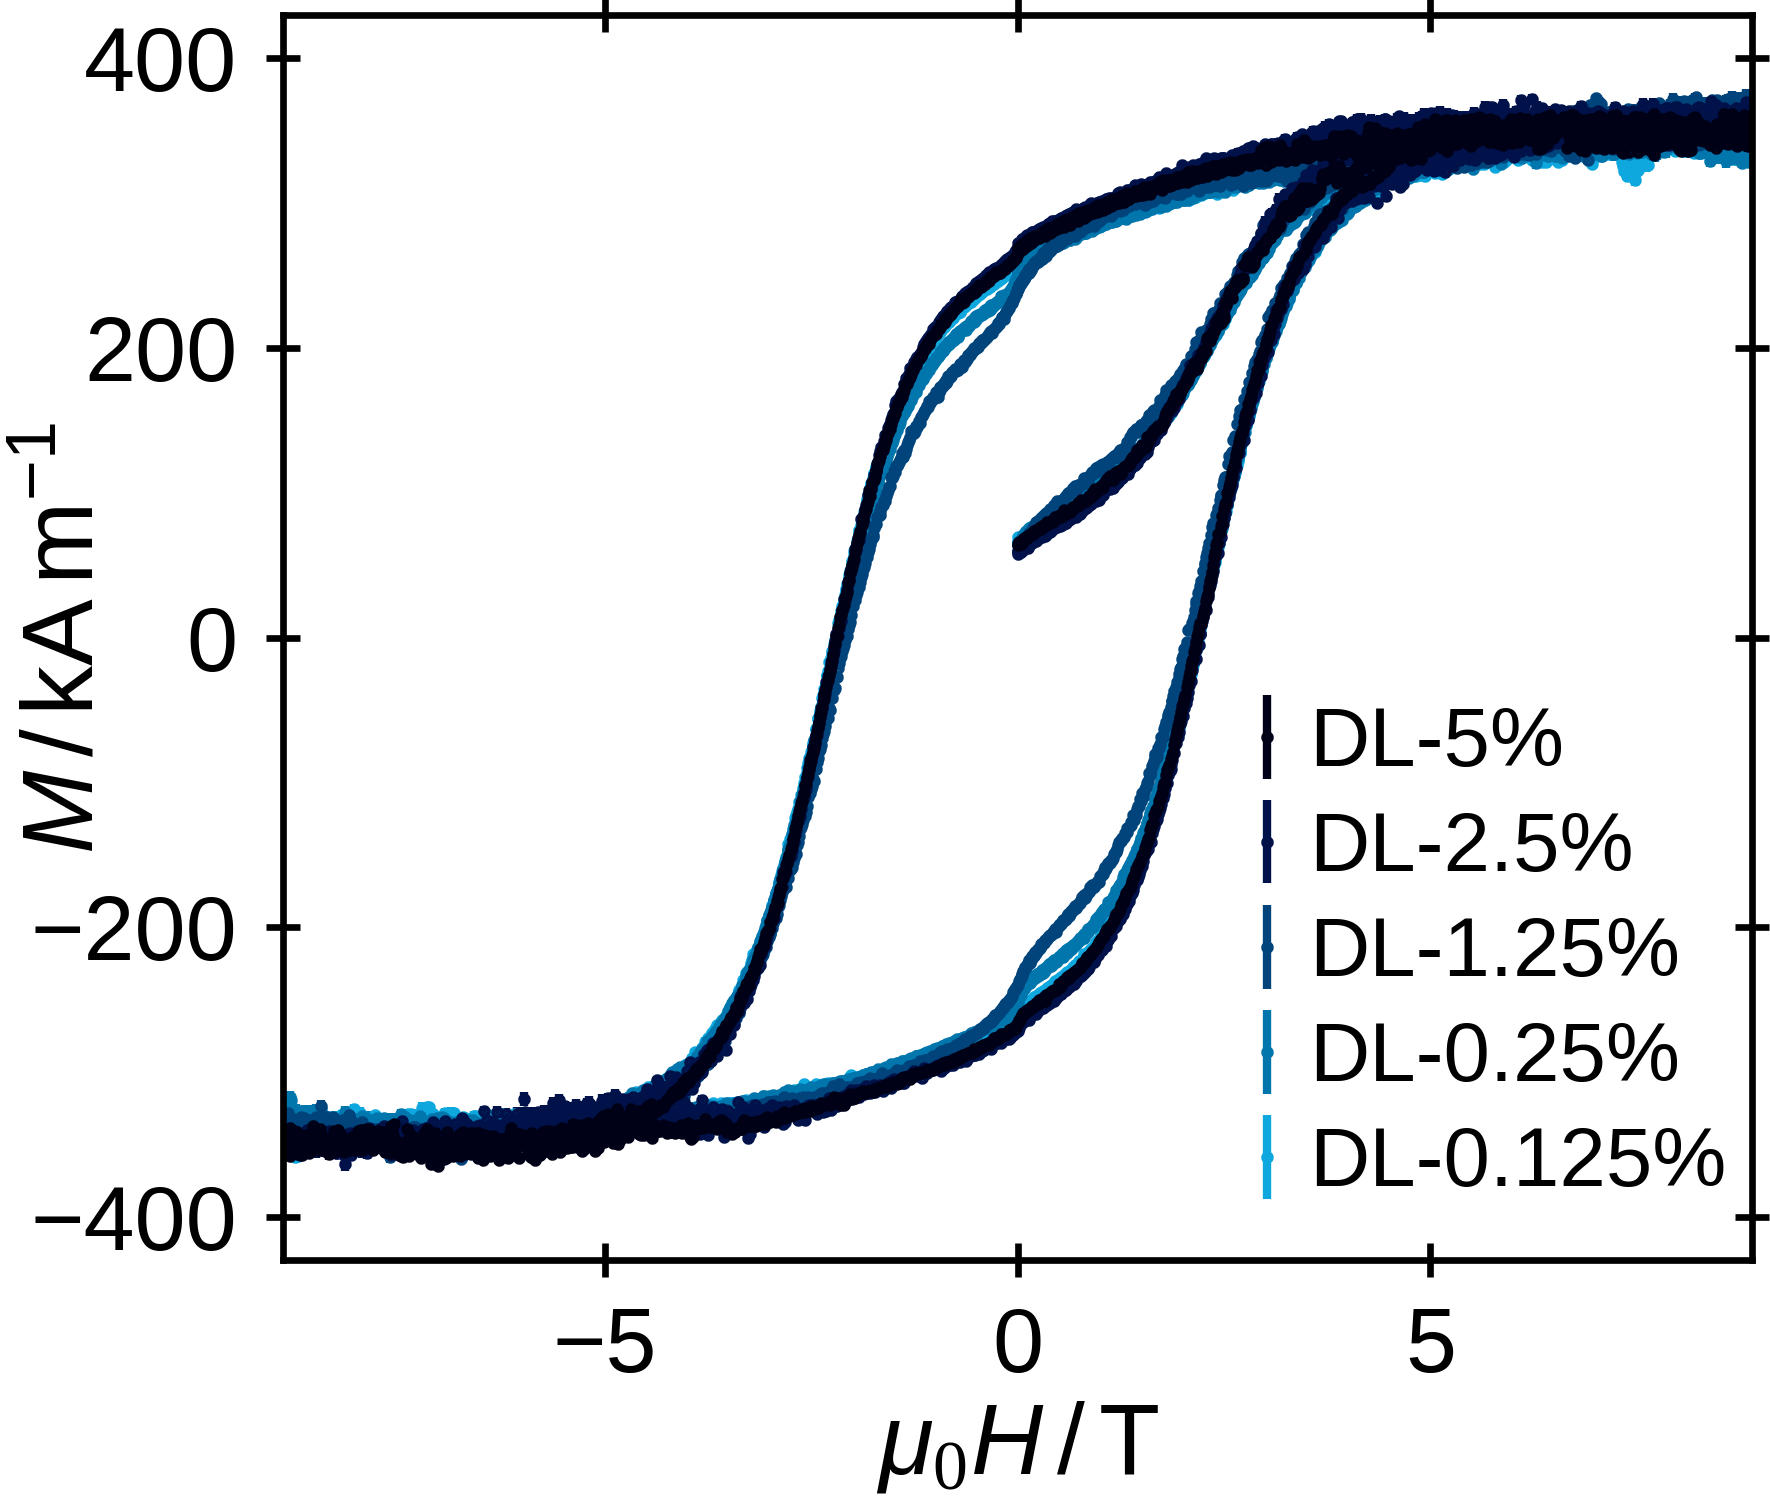
\includegraphics{doublelayers_PPMS_10K_allSamples}
    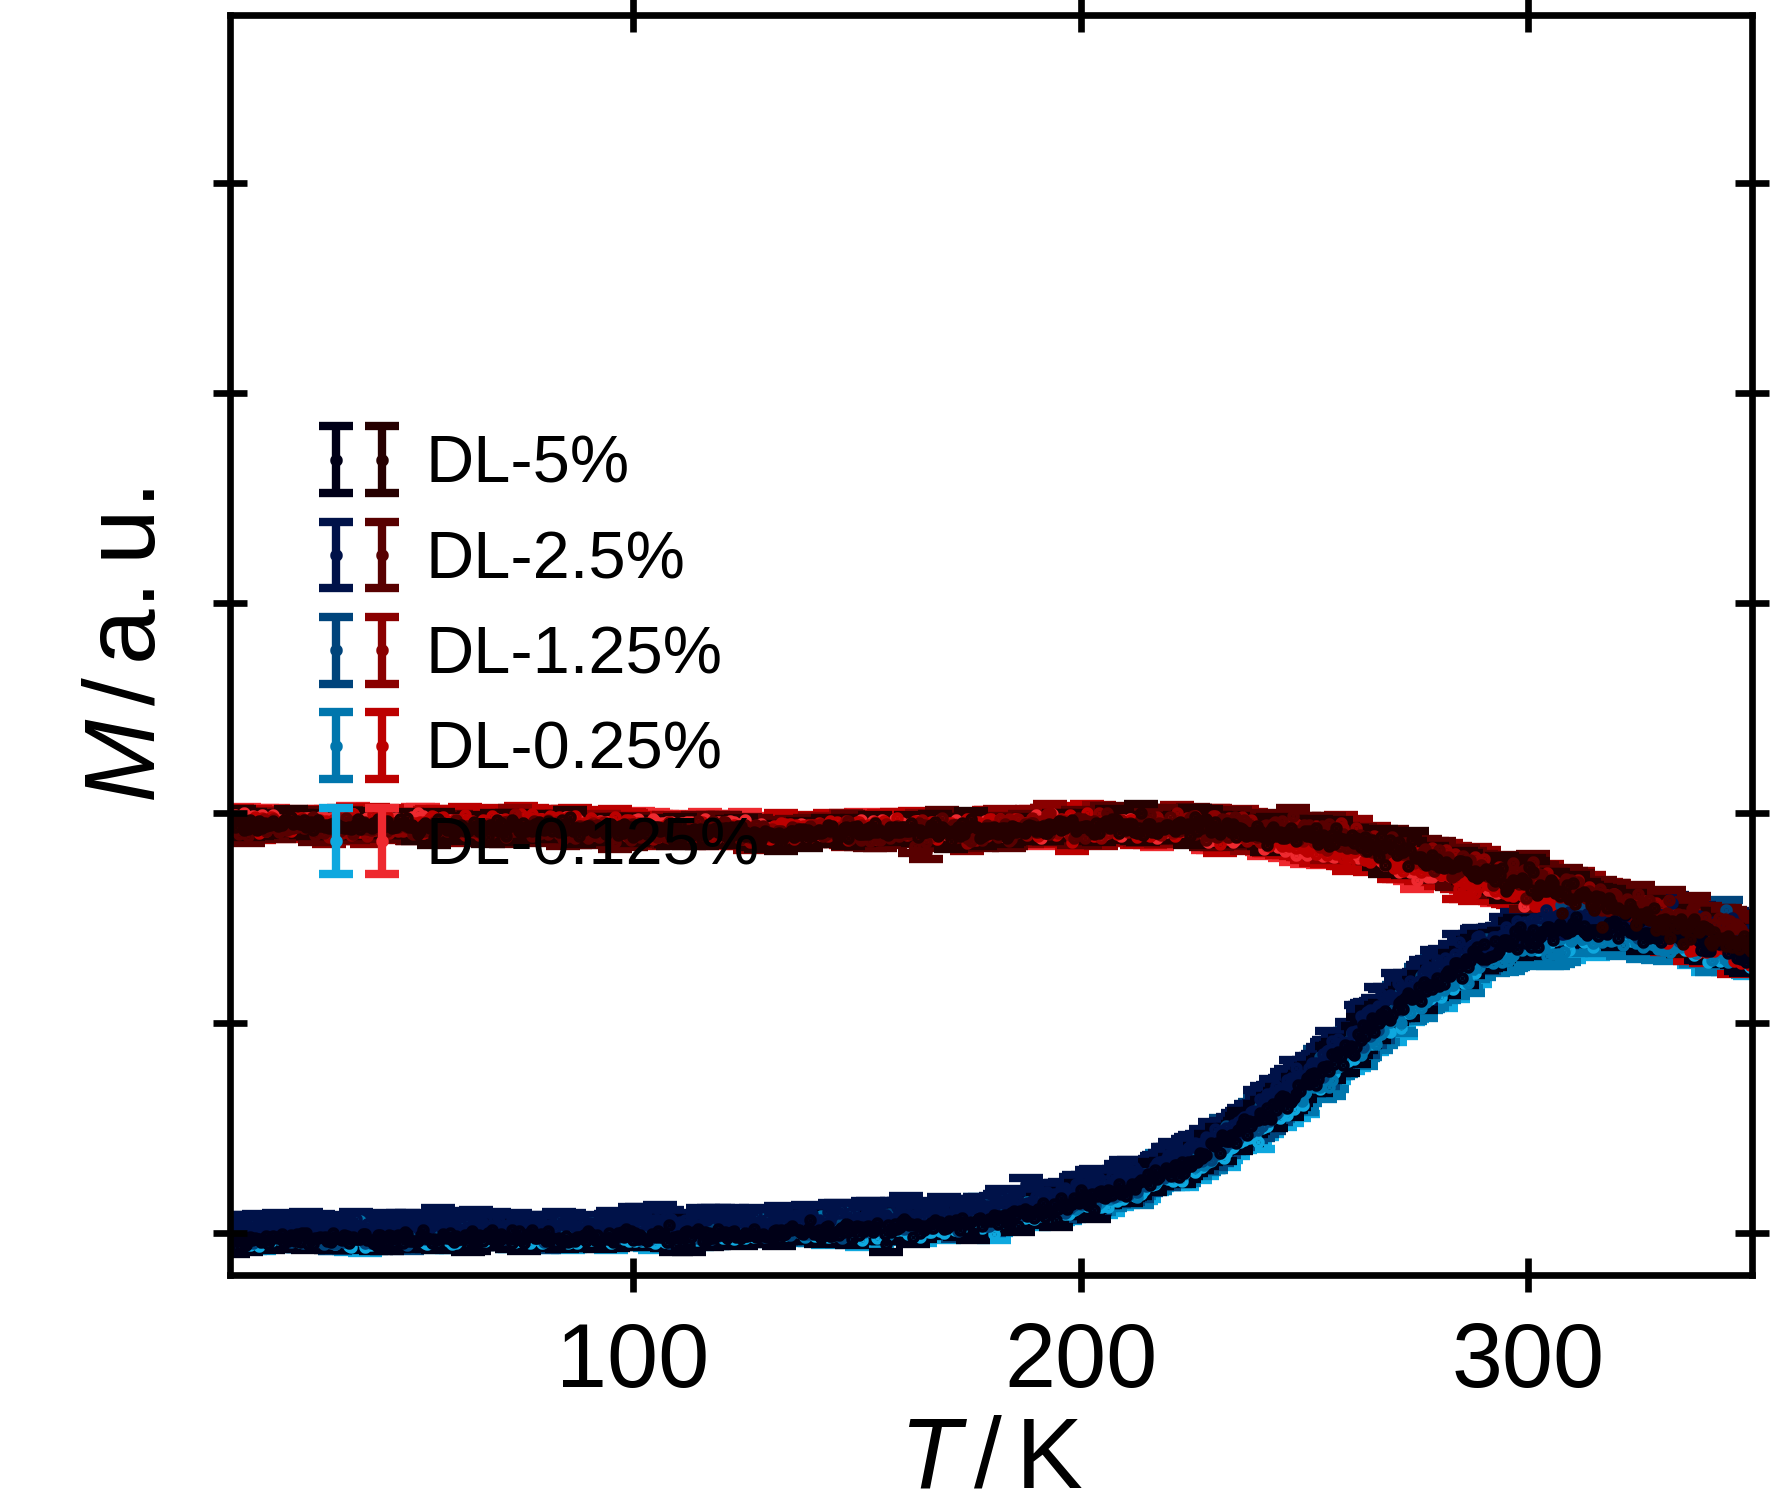
\includegraphics{doublelayers_PPMS_ZFC_FC_allSamples}
    \caption{\label{fig:doubleLayers:zfcFCData}Field- (left) and temperature-dependent (right) magnetization of the double layers. To discuss the qualitative differences, the zero-field cooled and field cooled data, as well as the respective data of the samples with varied spacer thicknesses are shifted by a constant factor.}
  \end{figure}

  % \begin{table}[!htbp]
  %   \centering
  %   \caption{\label{tab:looselyPackedNP:nanoparticle:gisaxs}Parameters for the hard-sphere structure factor in Percus-Yervick approximation shown in for both SC-IOS-11 and SC-IOS-7. $R_\mathrm{HS}$ is the hard-sphere radius and $\eta$ the packing fraction of the structure factor.}
  %   \begin{tabular}{ c | l | l }
  %     \rule{0pt}{2ex} \textbf{GISAXS}  & \textbf{SC-IOS-11} & \textbf{SC-IOS-7} \\
  %     \hline
  %     \rule{0pt}{2ex} $R_\mathrm{HS} \, / \unit{nm}$          & $5.655(2)$           & $3.872(4)$\\
  %     \rule{0pt}{2ex} $\eta          \, / \unit{\%}$          & $43.88(3)$           & $34.20(9)$\\
  %     \hline
  %   \end{tabular}
  % \end{table}
\end{document}